\chapter{Prototype implementation}
\label{cha:implementation}
This chapter discusses the prototype implementations of the tracker and the peer which will be evaluated in chapter \ref{cha:evaluation}. These implement the protocol designs from chapters \ref{cha:discovery} and \ref{cha:distribution}, and provide a working example of the protocol in action.

Section \ref{sec:impl:architecture} introduces the system architecture of the prototype. Section \ref{sec:impl:tracker} goes in-depth about the tracker's implementation, followed by the peer implementation in \ref{sec:impl:peer}. Some limitations of the prototype are outlined in \ref{sec:impl:limitations}, ending with a conclusion in section \ref{sec:impl:conclusion}.

\section{System architecture}
\label{sec:impl:architecture}

\subsection{Components}
Figure \ref{fig:impl:architecture} shows the types of components making up the NanoTorrent system. 

The tracker implementation is discussed in section \ref{sec:impl:tracker}. This is responsible for managing the swarms of all torrents, and providing information about these swarms to requesting peers through the NanoTracker protocol. It is assumed to run on a network outside of to the \gls{WSN}.

The peer implementation is detailed in section \ref{sec:impl:peer}. Peers must join the \gls{P2P} network, discover other peers, exchange information about available pieces and exchange missing pieces among each other. They communicate with each other through the NanoTorrent protocol.

A border router is needed to allow communications with the tracker since it is located on an external network. This border router provides the bridge between the \gls{6LoWPAN} communications on the \gls{WSN} and the pure \gls{IPv6} transmissions on the outside network. It also acts as the `root' node for the \gls{RPL} routing protocol used inside the \gls{WSN}. Since it is a common component in many \glspl{WSN} platform, it has a standard implementation in Contiki and is used as-is in the prototype architecture.

\begin{figure}
    \centering
    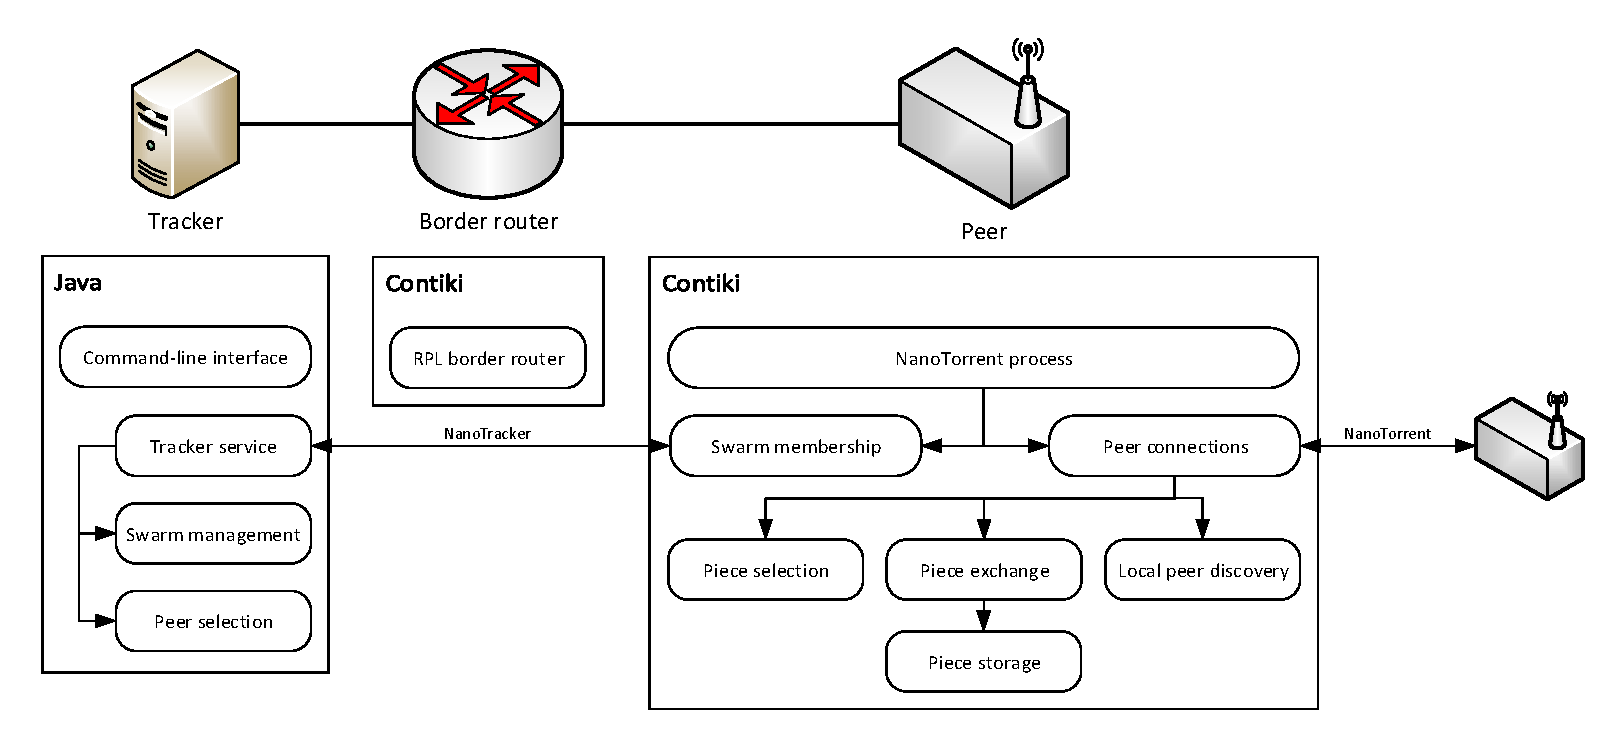
\includegraphics[width=\textwidth]{diagrams/protocol-architecture.pdf}
    \caption{NanoTorrent system architecture}
    \label{fig:impl:architecture}
\end{figure}

\subsection{Communications}
Figure \ref{fig:impl:protocol-overview} gives an overview of all protocol communications between these components in a \gls{WSN} infrastructure.

Peers start off by sending an announce request (1) to the tracker, which must be routed through the border router. The tracker replies with an announce reply (2) containing a list of peers to connect with.

From there, they can initiate peer connections with these discovered peers by sending an initial \texttt{have} message (3). They exchange information about available pieces, and send piece requests for missing pieces (4).

Peers can also discover neighbouring peers through local peer discovery (5), after which they can go through the same process of setting up a peer connection (6) and exchanging pieces (7).

\begin{sidewaysfigure}
    \centering
    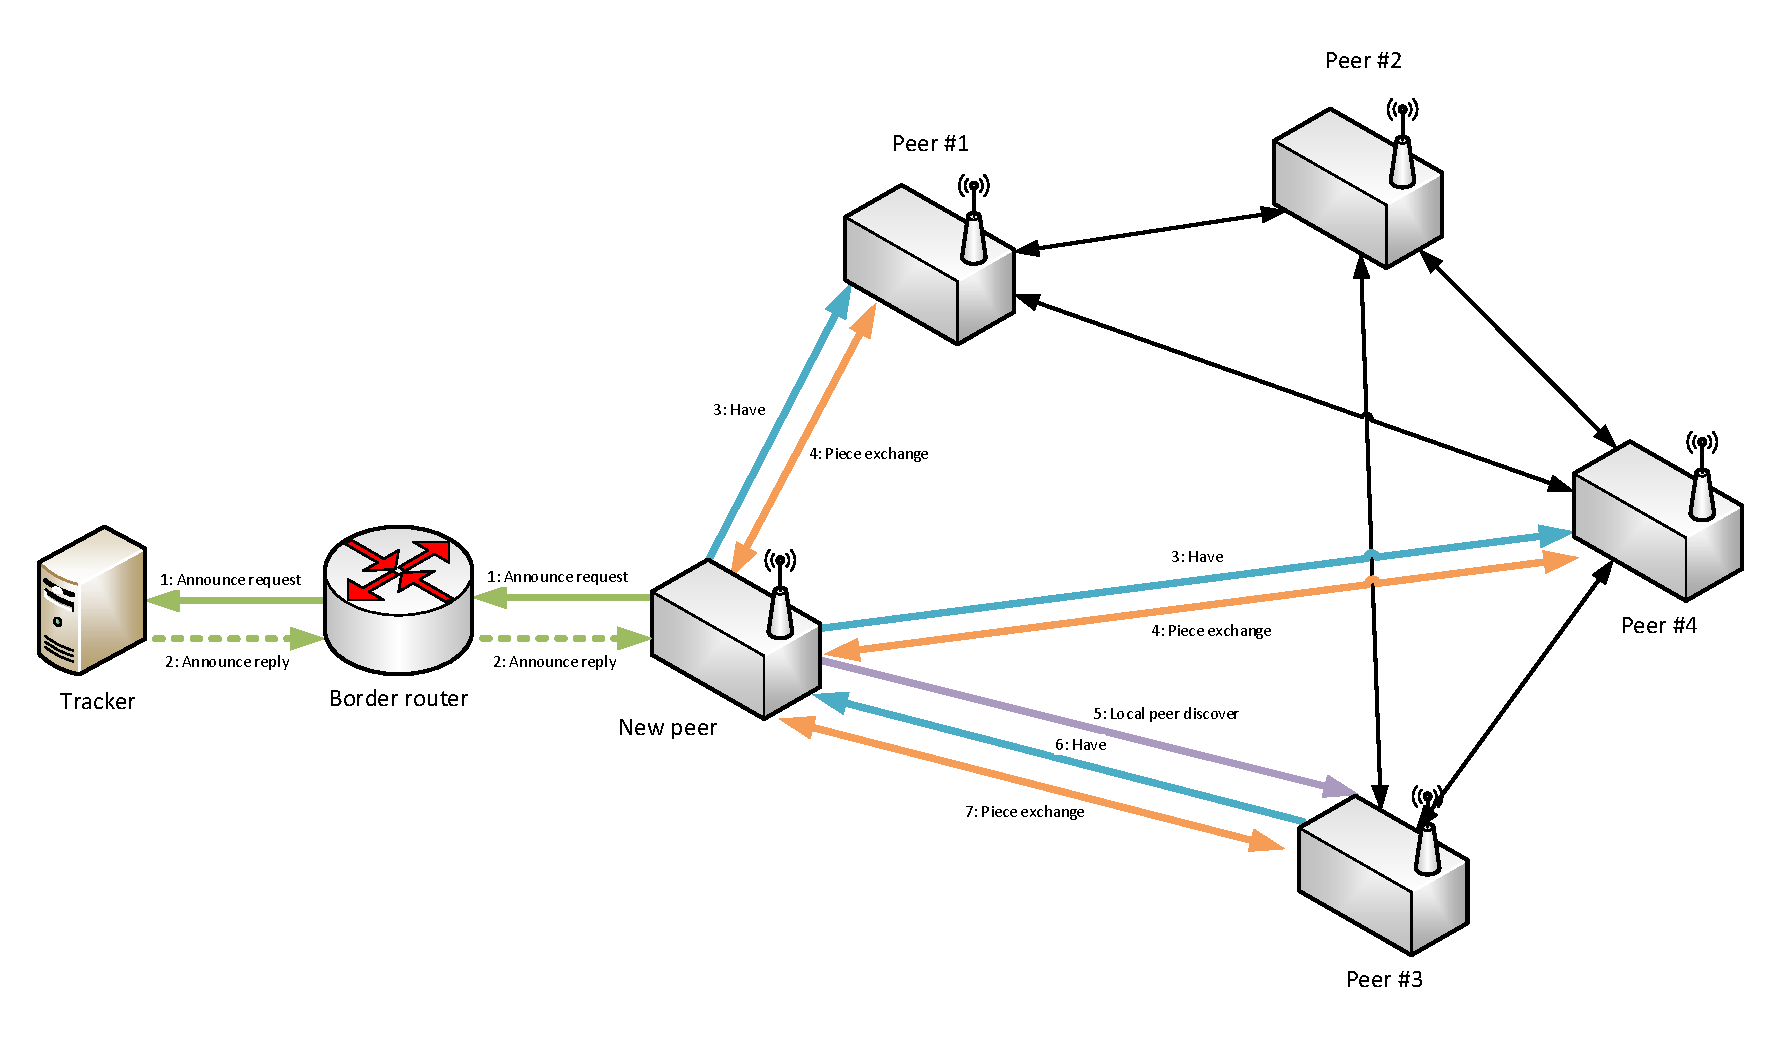
\includegraphics[width=\textwidth]{diagrams/protocol-overview.pdf}
    \caption{Overview of the NanoTorrent protocol communications in a \gls{WSN}}
    \label{fig:impl:protocol-overview}
\end{sidewaysfigure}

\section{Tracker}
\label{sec:impl:tracker}
The tracker described in section \ref{sec:discovery:tracker} is implemented as a standalone Java application. It starts a service to handle incoming NanoTracker announce requests, and provides a basic command-line interface to inspect its \glspl{swarm}.

Its implementation consists of a tracker service component for communications, a swarm manager to retain stateful information, and a peer selection algorithm to generate the peers lists for announce replies.

\subsection{Tracker service}
The tracker service provides the communication endpoint for peers wanting to join or leave a torrent's swarm. It is responsible for parsing incoming announce requests, triggering the needed operations in the managed swarms, collecting the information needed for the announce reply and then sending the reply.

The service listens on a user-specified \gls{UDP} port for incoming announce requests, which must be known by all peers wishing to communicate with this tracker. \gls{UDP} was chosen as underlying transport protocol rather than \gls{TCP}, as NanoTracker is a purely request-reply protocol with no need for long-term conversational state.

\subsection{Swarm management}
The tracker must manage stateful information about the torrent swarms that it is tracking. For every swarm, it retains information about the owning torrent (identified by its \gls{torrent-info-hash}) and the list of peers currently participating in the swarm. For every peer, the tracker records its \gls{IPv6} address, its current membership state and the time of the last received announce request.

When the tracker service receives a request for a torrent with an unknown \gls{torrent-info-hash}, it automatically creates a new swarm for that torrent to start tracking it. This is useful for quickly testing the prototype implementation: the tracker can just be started without any additional set up.

After looking up the swarm corresponding to the request's torrent, the tracker looks up the peer in the swarm based on its \gls{IPv6} address. If the peer is not yet in the swarm, it is added to it. The tracker updates its view on the peer's membership state using the reported state in the announce request, and refreshes the timestamp of its last announce request.

The tracker uses the timestamp of the last announce request sent by each peer to periodically purge non-responsive peers. When a peer fails to send its periodic announce requests to the tracker, its last announce timestamp does not get refreshed. The tracker can detect this and remove these peers. This ensures that peers will only discover peers that have recently refreshed their swarm state, and are likely to still be online when the peer tries to connect with them.

\subsection{Peer selection}
When the announce request is fully processed and the swarm's state is fully updated, the tracker service must reply to the request with a list of peers from the same swarm. This peers list is then used by the receiving peer to connect with other peers in the swarm.

In the current prototype, the tracker doesn't perform any special selection when generating the list of candidate peers. The tracker simply takes a random subset from the swarm, ensuring that this subset is no larger than the requested number of peers and does not include the requesting peer itself. A more intelligent selection algorithm could take advantage of additional information, for example it could prevent a seed from being connected to another seed (as these would have nothing to exchange with each other) or it could maintain a graph representation of the swarm to ensure that every peer is always directly or indirectly connected to a seed.

The generated peers list is used to construct an announce reply, which is then sent back to the peer by the tracker service.

\section{Peer}
\label{sec:impl:peer}
The peer implements the file distribution mechanisms described in chapter \ref{cha:distribution}, the requester's side of the centralized peer discovery from section \ref{sec:discovery:tracker} and the local peer discovery of section \ref{sec:discovery:local}. It is implemented in C on the Contiki platform \cite{contiki}, allowing for cross-compilation to many types of \gls{WSN} platforms.

\subsection{NanoTorrent process}
The main entry point for the peer's implementation is the NanoTorrent main process. This lightweight process initializes all other processes, such as the swarm process maintaining the connection with the tracker and the peer process maintaining connections with other peers. It also reads the list of peers retrieved from the swarm and uses them to initiate new peer connections.

\subsection{Swarm membership}
The swarm membership component is responsible for tracking the peer's membership state, maintaining the connection with the tracker (by periodically sending refreshes) and exposing the retrieved list of discovered peers to the main process.

The client starts a lightweight process to first join the swarm and then send periodic refreshes to the tracker. If it doesn't receive an announce reply after a number of retries, it assumes that the tracker has become unavailable or unreachable and marks itself as having left the swarm.

When the client discovers new peers through the tracker's announce replies, it temporarily stores them in a list while waiting for the main process to try and connect with them. The main process doesn't have to connect with all of the discovered peers, but can let the swarm process hold on to some of them until one of the current peer connections is lost and needs to be quickly replaced.

The main process is notified whenever the membership state changes, e.g. the client has successfully joined the swarm or when the client unexpectedly drops out of the swarm due to connection issues. These inter-process notifications ensure that the main process is aware of the state of all components, and can react when something goes wrong (e.g. losing the connection wit the tracker).

\subsection{Peer connections}
All peer connections and their messages are managed by the peer process. This process maintains a single \gls{UDP} socket listening on a fixed port (same for all NanoTorrent peers), parses the incoming peer messages and handles them for their various purposes: accepting new connections, responding to piece data request and discovering local peers. It is also responsible for the periodic \texttt{have} announcements to all connected peers.

The state that needs to be maintained for every peer connection is described in \ref{sec:distrib:connection}, and the used memory structures maintained by the process directly map onto this description. Peers keep track of the `heartbeat' of every connected peer using individual timers, which are refreshed on every received message. When a heartbeat timer expires, the peer drops the connection.

In order to keep the protocol scalable as the network size increases, peers limit the number of simultaneously opened peer connections. This prevents peers from opening or accepting too many connections, which all need network traffic and thus battery power to be maintained. The client uses two fixed-size `pools' for allocating peer connection states: one for incoming connections and one for outgoing connections. Rather than allocating memory for a new connection dynamically on the heap (e.g. using C's \texttt{malloc}), these pools are allocated in static memory and have a more predictable behaviour.

When a pool is exhausted, newly requested connections cannot be instantiated and these connections must be closed. However, exhaustion of one pool does not affect the other pool. For example, when a client initiates many outgoing connections with peers discovered locally, it can still accept incoming connections from other peers who discovered the client through the tracker.

\subsection{Piece selection}
Whenever a new peer connection is opened or an existing connection is updated with new information about available pieces, the peer process checks if it can request a missing piece on this connection.

Peers use a rarest-first policy for deciding which piece to select next, as described in \ref{sec:distrib:exchange}. To implement this, a client tracks the amount of occurrences of every piece at each of its peers, and finds the piece with the least amount of occurrences (excluding zero occurrences). Whenever a peer connects or disconnects, their available pieces are added or subtracted from the list of piece occurrences.

Peers make sure to not request the same piece from two connections at a time. This is managed in a shared variable, which is modified when new requests are made or old requests are finished. However, when a peer has received almost all of the pieces in a torrent, it is not desirable having to wait on just one peer to deliver the last piece. In this case, the peer goes into what BitTorrent calls \emph{end-game mode}: when nearing completion, a single piece may be requested from more than one connection. The impact of this is minimal as it only occurs at the very end of the download, but makes sure that peers can quickly transition from almost done to fully seeding.

\subsection{Piece exchange}
When a peer discovers an interesting piece at another peer, it can request this piece and start downloading it as detailed in section\ref{sec:distrib:exchange}.

Piece requests are managed individually per connection, with different retry counters and timers for the multiple outstanding requests. This allows parallel requests to operate independently from each other, preventing a single failing connection to take down all connections.

Piece replies destined to local neighbours are sent as multicast packets rather than unicast packets, as specified in \ref{sec:distrib:multicast}. Since the only change is in the destination \gls{IPv6} address, this is readily implemented as a small special case.

\subsection{Piece storage}
The piece data received in piece data replies is written to a file in the \acrfull{CFS}. The client uses the piece index and the piece data offset to calculate the byte offset in the file, and writes the bytes from the reply into the file. Similarly, data is read from the file when sending a piece data reply.

On the AVR Zigduino platform, \gls{CFS} is configured to use the \gls{EEPROM} for file system storage. This allows for 4 KB of read/write storage \cite{zigduino-manual}, which is sufficient for most network reprogramming or reconfiguration use cases. For experiments in the COOJA simulator \cite{cooja}, \gls{CFS} uses an in-memory file system.

\subsection{Local peer discovery}
Peer discovery through local multicast as discussed in section \ref{sec:discovery:local} is implemented as a modification to the periodic \texttt{have} announcements. Rather than sending the \texttt{have} announcements to individual local peers, it is multicasted to all local neighbours.

Incoming \texttt{have} multicast announcements are handled as regular incoming connection requests. The peer will try to accept the connection (if it hasn't already), and will process the message if it has a connection. As noted in \ref{sec:distrib:connection}, peers must not reply with a \texttt{close} message if it fails to accept a connection in response to a multicast \texttt{have}. Other than that, it can treat local peers and remote peers uniformly.

\section{Usage}
\label{sec:impl:usage}

\subsection{Deployment}
In order to deploy NanoTorrent onto a \gls{WSN}, the network operator must deploy the tracker on a computer on an external network, deploy a Contiki application using NanoTorrent onto the \gls{WSN} nodes and connect the external network with the \gls{WSN} with a border router.

\subsubsection{Tracker}
The tracker is a simple Java command-line application which can be started to operate on any \gls{UDP} port. The computer on which it is deployed must have a Java runtime installed and must have a connection with the border router. Other than that, the tracker is very much `fire and forget': it can run in the background and doesn't need user interaction.

\subsubsection{Peer}
The prototype is implemented in C for the Contiki platform, so it must be compiled for the particular platform used by the \gls{WSN} nodes. The implementation does not rely on hardware-specific features, so it can readily be cross-compiled to any of Contiki's supported platforms -- although it is recommended to fine-tune the protocol's configuration to the specifics of the used platform.

The prototype comes with a demo application, which has been verified to run on both the AVR Zigduino platform and in the COOJA simulator environment. The demo is implemented in \texttt{peer/demo.c} and can be compiled with the Makefile rule \texttt{demo}.

\subsubsection{Border router}
The \gls{RPL} border router is a standard component in Contiki, and can be found in \texttt{contiki/examples/ipv6/rpl-border-router}.

\subsection{Bootstrapping}
Before peers can start downloading a torrent, they must have received the \gls{torrent-desc} from the distributor, as explained in \ref{sec:discovery:torrent-desc}. The torrent descriptor is needed to `bootstrap' the NanoTorrent client, as it contains vital information needed for the file distribution. In the case of BitTorrent, the distributor creates and publishes a \texttt{.torrent} file containing the torrent's metainfo, as mentioned in section \ref{sec:related:bittorrent}. Users download this \texttt{.torrent} file and open it with a BitTorrent client to start the download.

\subsubsection{NanoGen toolchain}
The distributor can use the included NanoGen tool to generate a torrent descriptor file to be distributed to all destined NanoTorrent nodes. NanoGen takes as input the file to be distributed, details about the tracker and the piece size and produces a binary file which can be parsed by the NanoTorrent prototype implementation. The tool takes care of subdividing the input file into pieces of the given size, calculating the SHA-1 hashes of every piece and writing them to the output file.

To inspect the contents of a generated torrent descriptor file, the NanoRead utility was added. This utility takes a torrent descriptor file as input and prints its contents in a human-readable format. This is useful for verifying the contents of a generated or download torrent descriptor, and for debugging purposes.

NanoGen and NanoRead are implemented in C as Contiki applications in \texttt{peer/nanogen.c} and \texttt{peer/nanoread.c}. They can be compiled through the Makefile rules \texttt{nanogen} and \texttt{nanoread} with the flag \texttt{TARGET=native} to compile for the native platform (e.g. Linux). These rules produce executables for the command-line applications named \texttt{nanogen.native} and \texttt{nanoread.native}.

\subsubsection{Torrent descriptor distribution}
The current prototype implementation does not provide a mechanism for distributing a torrent descriptor. Like BitTorrent, the NanoTorrent client requires that the descriptor is available locally on the node, and is not concerned with \emph{how} the descriptor is retrieved.

For evaluation and demonstration purposes, the torrent descriptor is hard-coded into the NanoTorrent image at compilation time. The Makefile rule for the demo application takes a \texttt{TORRENT\_DESC} argument which specifies the path to the torrent descriptor file. This file is written in the static file system section of the created demo image, which will be read by the demo application at node start up.

\subsubsection{Seed configuration}
In order to configure a node act as a seed, it must have the whole file available at start up. NanoTorrent clients use the \acrfull{CFS} for storing the distributed file, so the seed must have the file prepared in its local file system.

On the AVR Zigduino platform, \acrfull{CFS} is configured to use the \gls{EEPROM} for file system storage. The Makefile provides the \texttt{demo.seed} rule to generate an \gls{EEPROM} image for the file system with the given \texttt{TORRENT\_FILE} at the start of the \gls{CFS} region. A seed can then be flashed with the \texttt{demo.seed.eu} and \texttt{demo.seed.u} rules.

For evaluating the NanoTorrent implementation in the COOJA simulator \cite{cooja}, the distributed file must be uploaded to the appropriate NanoTorrent nodes through COOJA's mote configuration interfaces.

\section{Limitations}
\label{sec:impl:limitations}
The current implementation is very much just a prototype. Many features common in mature file distributions are missing or are not fully fleshed out.

\subsection{Bootstrapping}
Currently, the torrent descriptor is hard-coded into the peer's program during compilation, locking the peer into downloading just one file. A more complete network reprogramming solution based on NanoTorrent should include a more versatile distribution mechanism for this descriptor.

The particularities of such mechanism depend heavily on the used \gls{WSN} middleware platform. For example, a \gls{WSN} running on the LooCI \cite{looci} platform would communicate mostly through LooCI's event-based communication network. A reconfiguration engine based on NanoTorrent for LooCI could send the torrent descriptor as payload data of a LooCI event, and have them launch the NanoTorrent process in response.

\subsection{Security}
The prototype assumes that nodes in the network can be trusted. Although this assumption is defendable in the context of experimental \glspl{WSN}, it does not hold for large-scale deployments where malicious peers could attack the network from the outside or the inside.

For example, a malicious node could intentionally send corrupted piece data to a peer, causing it to write the wrong data to its file. The peer will detect the corruption only after it has fully received the piece (possibly through multiple data requests), and will need to request the same piece again.

The tracker is also susceptible to uncontrolled announce requests. Every time a new request arrives for an unknown torrent, the tracker creates a new swarm and starts tracking it. This is sufficient for small-scale experimental uses, but could be abused by sending many announce requests with bogus torrent info hashes. The tracker would allocate a lot of swarms which are never used and never cleaned up, potentially crashing it due to it running out of memory. To prevent such abuse, trackers deployed in the wild should only accept announce requests for known torrents registered in a backing database.

\section{Conclusion}
\label{sec:impl:conclusion}
The prototype for the tracker and the peer provides the basic implementation of the protocol designs from chapters \ref{cha:discovery} and \ref{cha:distribution}, taking into account the constraints and limitations imposed by \gls{WSN} nodes. It comes with tools for generating and inspecting torrent descriptors, monitoring the swarms on the tracker and compiling images for NanoTorrent leechers and seeds.

The prototype lacks additional features commonly found in more mature file distribution mechanisms, such as an easy-to-use bootstrapping process or security checks. However, it provides enough to do useful evaluations of the proposed protocol in small experiments.
